\documentclass[12pt,a4paper,oneside,brazil]{abntex2}
\usepackage[utf8]{inputenc}
\usepackage[T1]{fontenc}
\usepackage[brazil]{babel}
\usepackage{graphicx}
\usepackage{lipsum} % Pacote para gerar texto fictício
\usepackage{helvet}
\usepackage{ragged2e}
\usepackage{glossaries}
\usepackage[alf]{abntex2cite} % Citações padrão ABNT
\usepackage{indentfirst}

\setlength{\parindent}{1.5cm}

\renewcommand{\familydefault}{\sfdefault}

\hypersetup{
    hidelinks
}

\titulo{Plataforma de Edição/Automação para trabalhos acadêmicos}
\autor{Higor Ferreira Alves Santos}
\orientador{Marcelo Antônio Adad}

\newcommand{\ies}{Pontifícia Universidade Católica de Goiás}
\newcommand{\escola}{Escola Politécnica e de Artes}
\newcommand{\curso}{Engenharia de Computação}

\newcommand{\grauOrientador}{Prof. M.E.E.}
\newcommand{\grauAluno}{Bacharel}

\newcommand{\grauBancaUm}{Prof. Dra.}
\newcommand{\bancaUm}{Miriam Gusmão}
\newcommand{\grauBancaDois}{}
\newcommand{\bancaDois}{}

\instituicao{%
    \ies
    \par
    \escola
    \par
    \curso
    }
\local{GOIÂNIA - GO}
\data{2023}


\newglossary*{abrev}{Lista de abreviaturas}
\newglossary*{siglas}{Lista de siglas}
\newglossary*{simbolos}{Lista de símbolos}

\newglossaryentry{termo1}{
    type=abrev,
    name={Termo 1},
    description={Descrição do termo 1}
}

\newacronym[type=siglas]{abnt}{ABNT}{Associação Brasileira de Normas Técnicas}
\newacronym[type=siglas]{ue}{UE}{União Européia}

\newacronym[type=simbolos]{dollar}{\$}{Dollar americano}

\makeglossaries


% Início do documento
\begin{document}

\renewcommand{\listfigurename}{Lista de Figuras}
% Alterando o título da lista de tabelas
\renewcommand{\listtablename}{Lista de Tabelas}
% Alterando o título do sumário
\renewcommand{\contentsname}{Sumário}

% Capa personalizada
\begin{capa}
    \center

    \OnehalfSpacing
    \ABNTEXchapterfont\bfseries{\textsc{\MakeUppercase{\imprimirinstituicao}}}

    \vfill

    % Incluir logotipo
    
\includegraphics[width=0.15\textwidth]{./src/assets/logo.png}

    \vfill

    \ABNTEXchapterfont\bfseries{\MakeUppercase{\imprimirtitulo}}

    \vfill

    \MakeUppercase{\imprimirautor}

    \vfill

    \bfseries{\MakeUppercase{\imprimirlocal}}

    \bfseries{\MakeUppercase{\imprimirdata}}
\end{capa}

% Folha de rosto personalizada
\begin{folhaderosto}

    \centering

    \MakeUppercase{\imprimirautor}

    \vfill

    \ABNTEXchapterfont\bfseries{\MakeUppercase{\imprimirtitulo}}

    \vfill

    \justifying
    \noindent\hspace*{70mm}%
    \begin{minipage}{\dimexpr\textwidth-70mm}
        \textnormal{
            Trabalho de Conclusão de Curso apresentado à
            \escola, da \ies, como parte dos
            requisitos para a obtenção do título de \grauAluno\,em
            \curso.\\\\
            Orientador:\\
            \begin{flushright}
                \grauOrientador \imprimirorientador
            \end{flushright}
            Banca examinadora:\\
            \begin{flushright}
                \grauBancaUm \, \bancaUm
                \grauBancaDois \, \bancaDois
            \end{flushright}
        }
    \end{minipage}

    \vfill

    \centering

    \bfseries{\imprimirlocal}

    \bfseries{\imprimirdata}
\end{folhaderosto}

% Folha de aprovação
\clearpage
    \centering
    \MakeUppercase{\imprimirautor}

    \vfill

    \ABNTEXchapterfont\bfseries{\MakeUppercase{\imprimirtitulo}}

    \vfill

    \justifying

    \textnormal{Trabalho de Conclusão de Curso aprovado em sua forma final pela Escola Politécnica e de
    Artes, da Pontifícia Universidade Católica de Goiás, para obtenção do título de \grauAluno\,em
    Engenharia de Computação, em: \rule{8mm}{0.4pt}/ \rule{8mm}{0.4pt}/ \rule{16mm}{0.4pt}}

    \centering

    \vspace*{3cm}

    \begin{flushright}
    \rule{10cm}{0.4pt}\\
    \textnormal{Orientador: \grauOrientador \imprimirorientador}

    \vspace*{10mm}

    \rule{10cm}{0.4pt}\\
    \textnormal{Orientador1: \grauBancaUm \, \bancaUm}

    \vspace*{10mm}

    \rule{10cm}{0.4pt}\\
    \textnormal{Orientador2: \grauBancaDois \, \bancaDois}
    \end{flushright}

    \vspace*{6cm}

    \bfseries{\imprimirlocal}

    \bfseries{\imprimirdata}
\clearpage % Começa uma nova página para a folha de rosto

%Dedicatória
\centering
\ABNTEXchapterfont\bfseries{\textsc{\MakeUppercase{Dedicatória}}}\\
\vspace*{3cm}
\justifying
\normalfont
\lipsum[1-5]
\clearpage

%Agradecimentos
\centering
\ABNTEXchapterfont\bfseries{\textsc{\MakeUppercase{Agradecimetos}}}\\
\vspace*{3cm}
\justifying
\normalfont
\lipsum[1]
\clearpage

%Epígrafe
\centering
\ABNTEXchapterfont\bfseries{\textsc{\MakeUppercase{Epígrafe}}}\\
\vspace*{3cm}
\justifying
\normalfont
\lipsum[1-3]
\clearpage

%Resumo
\centering
\ABNTEXchapterfont\bfseries{\textsc{\MakeUppercase{Resumo}}}\\
\vspace*{3cm}
\justifying
\normalfont
\lipsum[12-13]
\clearpage

%Abstract
\centering
\ABNTEXchapterfont\bfseries{\textsc{\MakeUppercase{Abstract}}}\\
\vspace*{3cm}
\justifying
\normalfont
\lipsum[7]
\clearpage

\pagenumbering{roman}

\listoffigures   % Lista de Figuras
\clearpage

\listoftables    % Lista de Tabelas
\clearpage

\printglossary[type=abrev,title=Lista de Abreviaturas]
\clearpage

\printglossary[type=siglas,title=Lista de Siglas]
\clearpage

\printglossary[type=simbolos,title=Lista de Símbolos]
\clearpage

% Correção: Usar \tableofcontents para o Sumário
\tableofcontents
\clearpage



\pagenumbering{arabic}
\setcounter{page}{1}
\textual

\justifying
\normalfont

\chapter{Introdução}
Este é um exemplo de texto com uma nota de rodapé.\footnote{Aqui está o texto da nota de rodapé.} \lipsum[1]

\section{Caracteres especiais}
\#     \$     \%     \textasciicircum     \&     \_     \{     \}     \textasciitilde     \textbackslash \\
â ã
\\
\\
There is \# A house \%\%\%\\
In new Orleans \textasciicircum \\
Ç \textasciicircum \\
i neeedddd very mech \$\$\$\$\$\$\$\$\$\\
\$ \& CACHAÇA para mim\\
My \_\_\_\_\_\_\_\_\_\_\_\_\_\_ fucking\\
function () \{\}\\
\textasciitilde What'sapp text\textasciitilde  for me \textbackslash\\\\

\section{Subtítulo de Nível 1}
Texto com outra nota de rodapé.\footnote{Outro exemplo de nota de rodapé.} \lipsum[2-3]

\subsection{Subtítulo de Nível 2}
\lipsum[4]
\subsubsection{Subtítulo de Nível 3}
\lipsum[5]
\subsubsubsection{Subtítulo de Nível 4}
\lipsum[5]
% \subsubsubsubsection{Subtítulo de Nível 5}
% \subsubsubsubsubsection{Subtítulo de Nível 6}

\subsection{Subtítulo de Nível 2 de novo}

\chapter{Revisão da Literatura}
\lipsum[6-7]

\chapter{Teste de abreviaturas}
\section{Abrev 1}
\subsection{Abreviatura completa, (Primeira ocorrência)}
\gls{abnt}
\subsection{Segunda ocorrência}
\gls{abnt}
\subsection{Abreviatura crua, (acrshort)}
\acrshort{abnt}
\subsubsection{Crua com texto}
\acrshort{abnt} - Associação Brasileira de Normas Técnicas.
\subsection{Usando glsentryshort}
\glsentryshort{abnt}

\section{Abrev 2}
\gls{ue} - União européia

\section{Termo}
\gls{termo1}\\
\gls{termo1}\\
\acrshort{termo1}

\section{Símbolo}
\gls{dollar}\\
\gls{dollar} \\
Quero ganhar\acrshort{dollar}

\chapter{Matemática}
É muito fácil digitar equações em latex!\\
\lipsum[1][1-12]
\section{Equação inline}
$E=mc^2$\\\\
\lipsum[12][1-33]
\section{Equação centralizada}
$$E=mc^2$$

\section{Física}
\textbf{Relação de transformação}
$L=\text{Indutância;}\quad N=\text{Número de espiras;}\quad V=\text{Tensão}$

\textbf{Relação:}
$I=\Large\frac{L_1}{L_2}\normalsize=\left( \Large\frac{N_1}{N_2} \right)^2\normalsize=\left(\Large\frac{V_1}{V_2} \right)^2$

\textbf{Resistência:}
$R=\rho\Large\frac{L}{A}$

\textbf{Lei de Joule:}
$P=I^2R$

$\Large\frac{\frac{1}{60}}{\frac{\alpha}{1}}\normalsize=\Large\frac{1}{60\alpha}$

\chapter{Metodologia}
\lipsum[8-9]

\chapter{Citações}
\cite{hawking1988}\\
\cite{feynman1963}\\
\cite{douglas2004}\\
\cite{knuth1997}\\
\cite{orwell1984}\\
\cite{einstein1935}\\
\cite{shannon1948}\\
\cite{latexWiki}\\
\cite{pythonOrg}\\
\cite{smith1992}\\
\\\\
Conforme discutido na Wikipedia \cite{luaWikipedia}...\\
Em outro artigo da Wikipedia \cite{terraWikipedia}...\\\\
\cite{exemploCincoAutores}\\
Conforme \cite{hi}, a história se repete.


\chapter{Resultados e Discussão}
\lipsum[10]
\gls{abnt}

\begin{figure}[ht]
    \centering
    \caption{Exemplo de Figura}
    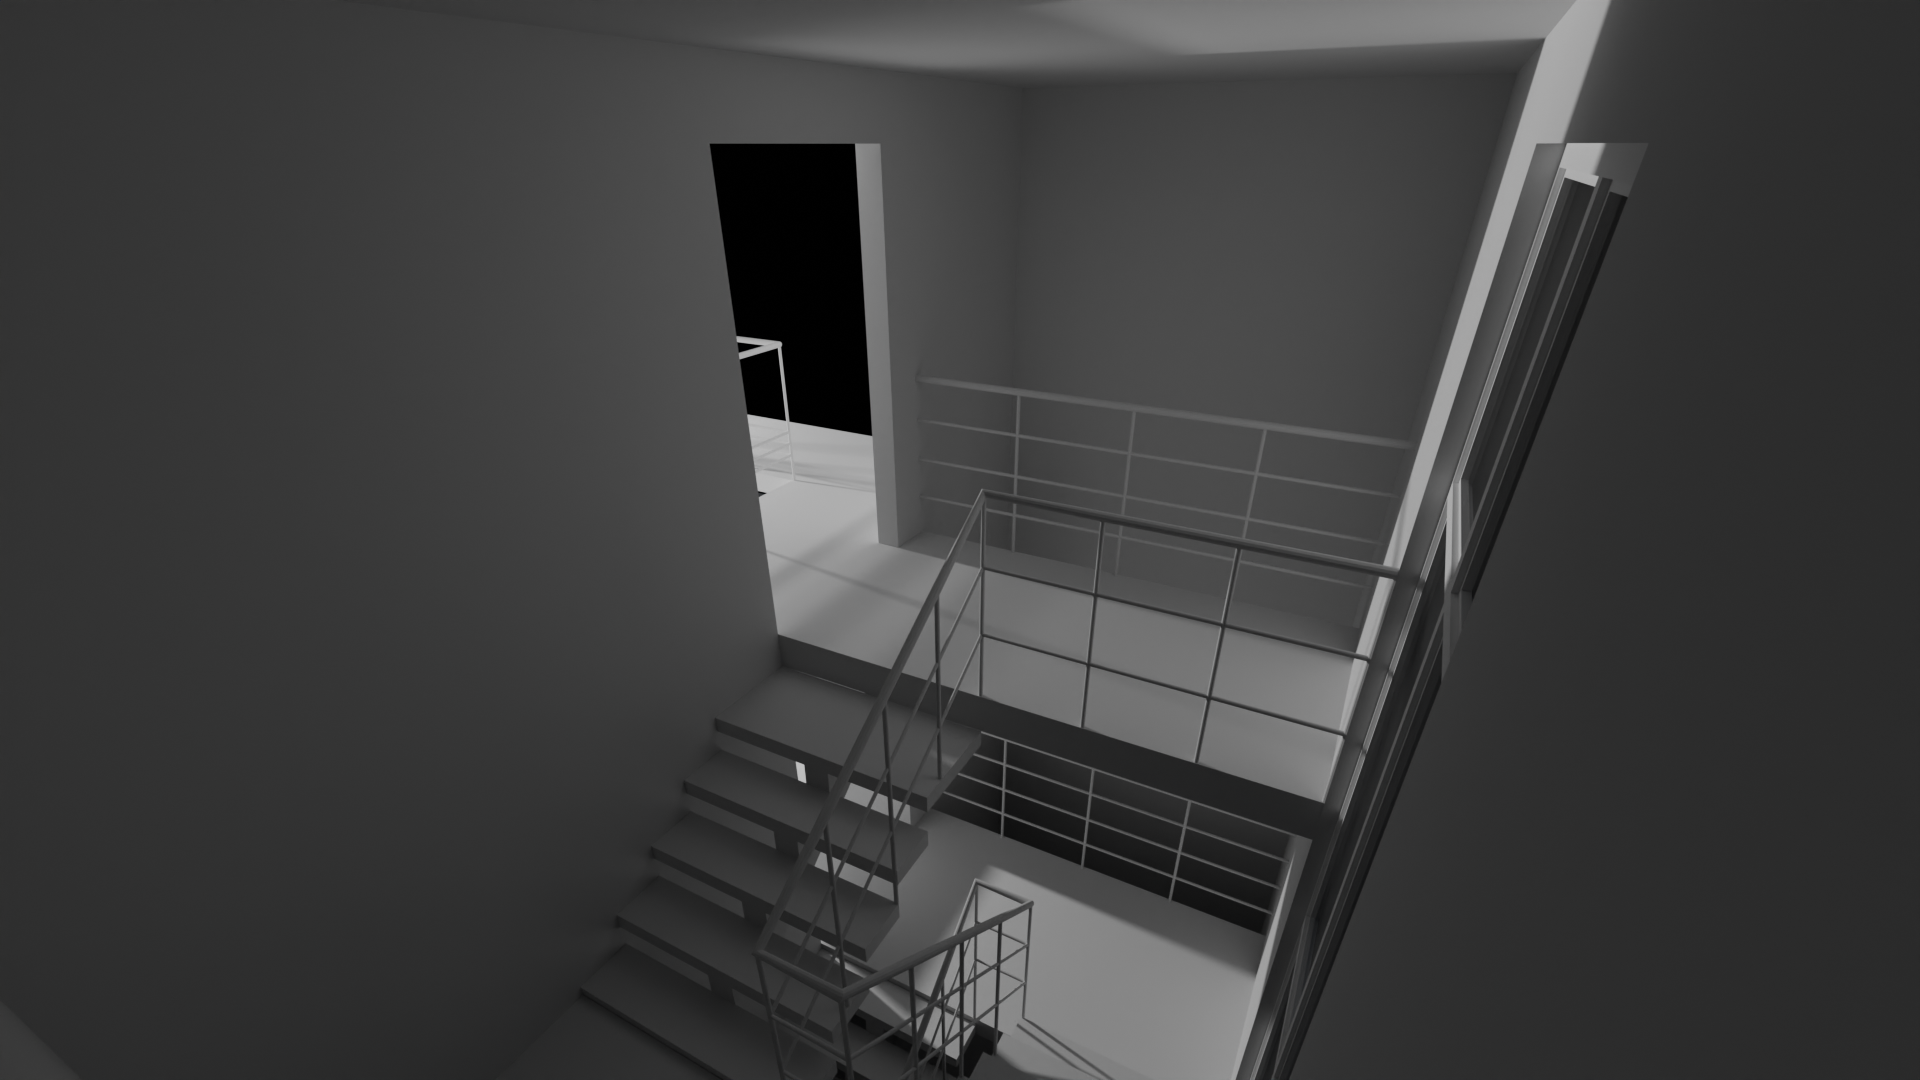
\includegraphics[width=1.0\textwidth]{./src/assets/untitled.png}
    \label{fig:exemplo}
    \textnormal{\fontsize{10pt}{12pt}Fonte: Autoria própria}
\end{figure}

\begin{table}[ht]
    \centering
    \caption{Exemplo de Tabela}
    \begin{tabular}{|c|c|c|}
        \hline
        Coluna 1 & Coluna 2 & Coluna 3 \\ \hline
        Item 1   & Item 2   & Item 3   \\ \hline
        Item 4   & Item 5   & Item 6   \\ \hline
    \end{tabular}
    \label{tab:exemplo}
    \\\textnormal{\fontsize{10pt}{12pt}Fonte: Autoria própria}
\end{table}

\lipsum[1-2]

Gostou? veja de novo a figura \ref{fig:exemplo}\\\\
(\acrshort{ue})

\chapter{Conclusão}
\lipsum[11-12]

\bibliography{referencias}

\end{document}